\chapter{Criação de redes locais}\label{chp:redesCompletas}
%%%% Baseado na https://www.youtube.com/watch?v=2gva8vJpHD0
Agora que já conhecemos como criar uma rede simples, passaremos a criar uma rede local um pouco mais complexa. Essa rede local terá componentes cabeados e componentes sem fio (\textit{wireless}). Além disso, introduziremos o uso do \textit{Dynamic Host Configuration Protocol} (DHCP). O DHCP é um protocolo de serviço TCP/IP que oferece configuração dinâmica de terminais, com a atribuição dinâmica de endereços IP e máscara de sub-rede, \textit{gateway} padrão, número IP de um ou mais servidores DNS e sufixos de pesquisa do DNS, entre outras informações.

\section{Topologia da Rede local}\label{sec:testeSec}
Na topologia que vamos criar, ilustrada na \Cref{fig:topDHCP}, utilizaremos os seguintes equipamentos:
\begin{itemize}
    \item Quatro PCs, três \textit{laptops} e uma impressora.
    \item Um \textit{switch} (2960-24T) que vai conectar três dos cinco PCs e a impressora.
    \item Um roteador sem fio (\textit{wireless router} WRT300N) para conectar dois dos cinco PCs e os \textit{laptops} (sem fio).
\end{itemize}

\begin{figure}[!hbt]
    \centering
    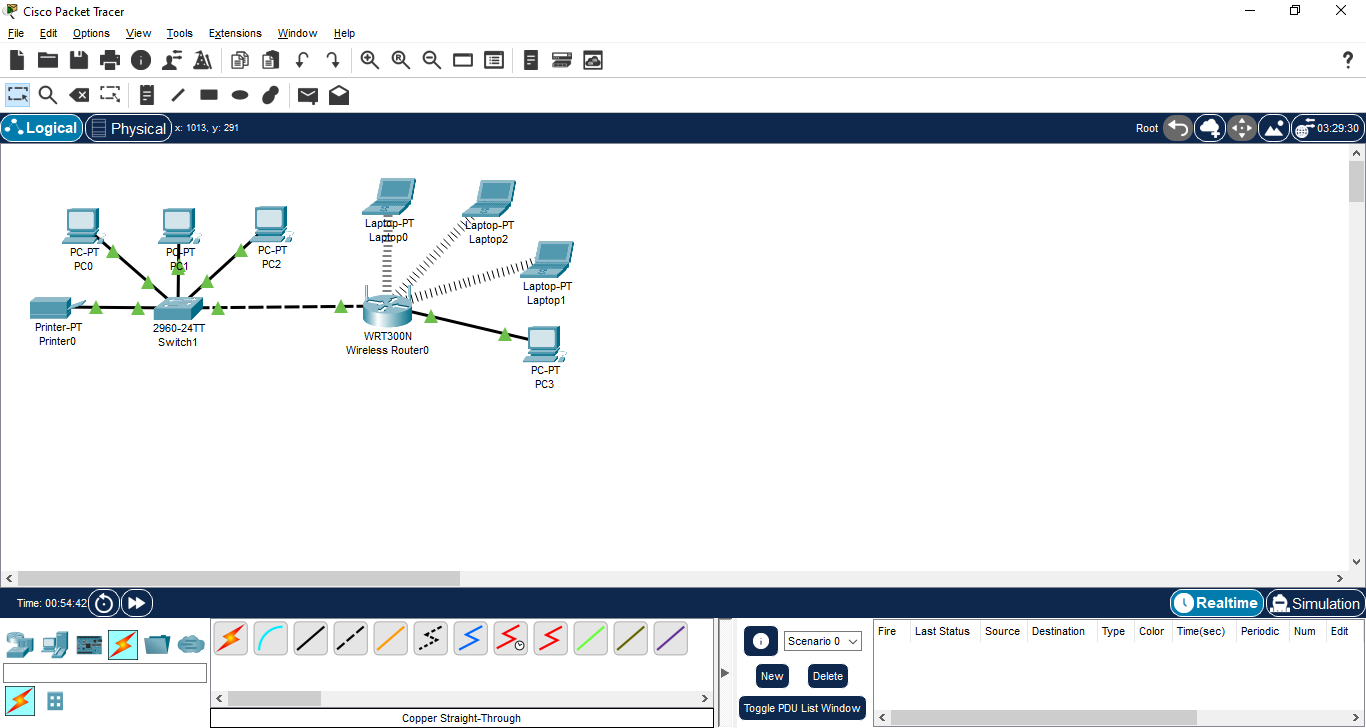
\includegraphics[width=.99\textwidth]{Figuras/RedeCompleta1}
    \caption{Topologia para rede local com DHCP.}\label{fig:topDHCP}
\end{figure}

Agora, vamos configurar essa rede local para que os equipamentos usem o DHCP para configuração automática dos seus endereços. Lembrando que  a impressora deve ter um IP fixo (\texttt{192.168.0.10}) e os demais equipamentos devem ter endereços dinâmicos atribuídos pelo DHCP.

Antes de começar, verifique se o cabeamento entre o \textit{switch} e o roteador sem fio é feito com um cabo \textit{cross-over}. Certifique-se também que os \textit{laptops} tenham placas para rede sem fio. Eles devem usar o módulo PT-LAPTOP-NM-1W-AC. Para instalar esse módulo (placa de rede) em um \textit{laptop}, execute os passos a seguir e observe a \Cref{fig:perfilLaptop}:

\begin{enumerate}[label*=\arabic*.]
  \item Clique sobre o ícone do \textit{laptop}.
  \item Na aba \textit{Physical}, você verá o perfil do \textit{laptop}. Desligue o equipamento, clicando no botão de liga/desliga (no canto esquerdo inferior da figura do \textit{laptop}).
  \item Arraste a placa de rede para a lista de módulos no canto esquerdo.
  \item Na lista de módulos, selecione o módulo PT-LAPTOP-NM-1W-AC e arraste para o local onde estava a placa de rede no \textit{laptop}.
\end{enumerate}

\begin{figure}[!hbt]
    \centering
    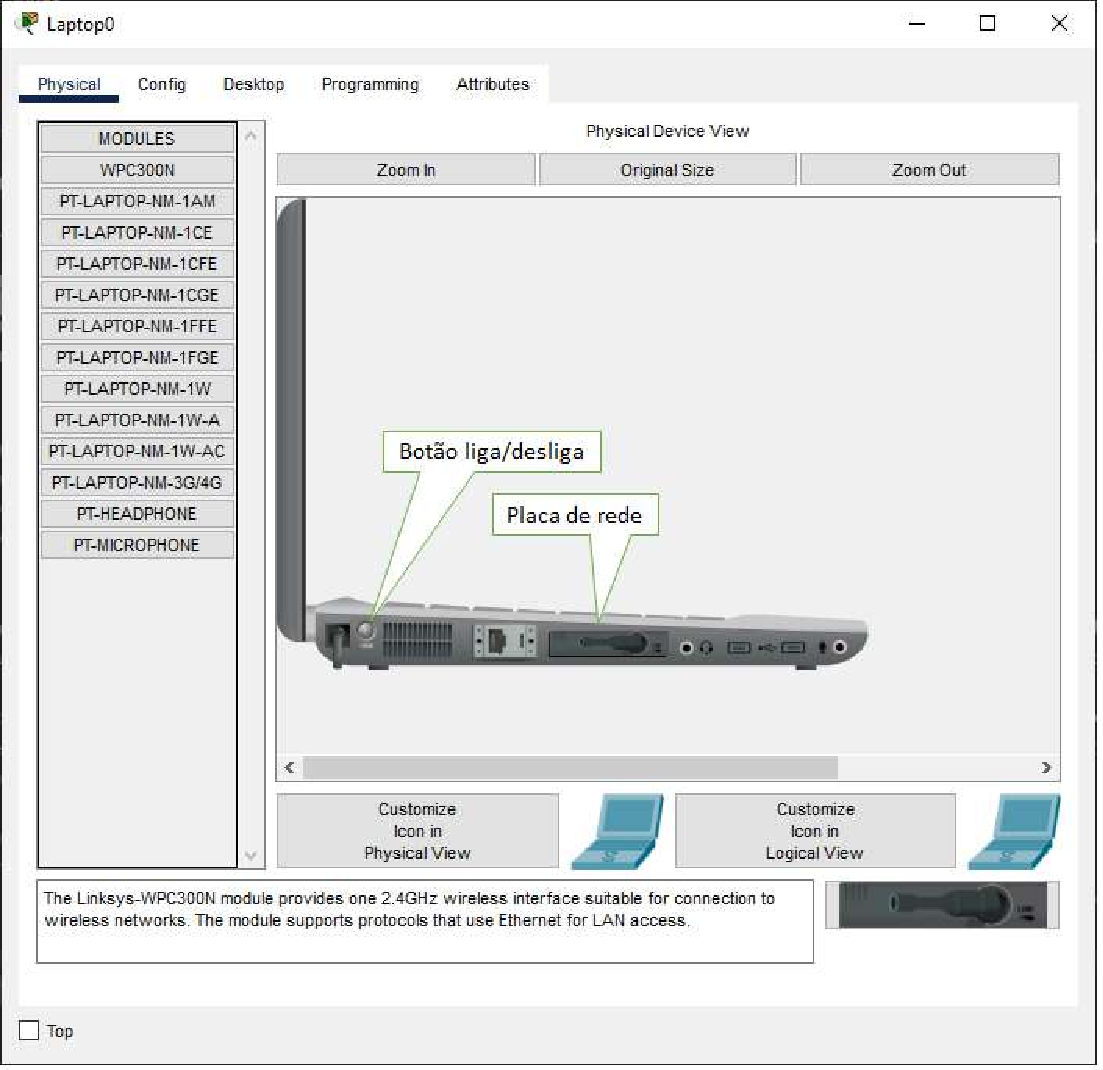
\includegraphics[scale=.8]{Figuras/PerfilLaptop}
    \caption{Perfil do \textit{laptop} para substituição da placa de rede sem fio.}\label{fig:perfilLaptop}
\end{figure}

\section{Configuração do roteador sem fio com DHCP}
Em redes sem fio, a utilização do DHCP é geralmente necessária, pois muitas vezes, há vários equipamentos que vão se ligar a essa rede. Assim, os equipamentos poderão ter suas configurações realizadas automaticamente. Realizaremos a seguir a configuração do DHCP no próprio roteador sem fio WRT300N. Os passos são os seguintes:

\begin{enumerate}[label*=\arabic*.]
  \item Clique sobre o ícone do roteador sem fio WRT300N.
  \item Na aba GUI, você verá a configuração inicial. Certifique-se que está na aba \textit{Setup} e com a opção \textit{Automatic Configuration -- DHCP} em tela.
  \item Identifique o \texttt{IP Address} do roteador. Ele já deve estar com o endereço IP \texttt{198.0.0.1} e máscara \texttt{255.255.255.0}.
  \item Confirme que o \texttt{DHCP server} está habilitado (\textit{Enable}).
  \item Agora, defina o endereço IP inicial (por padrão se inicia em 100) e o número máximo de usuários. Com isso, todos os novos usuários terão seus IPs a partir do endereço especificado. 
\end{enumerate}

Não esqueça de clicar no botão \textit{Save Settings} na parte inferior da tela. Use a barra de rolagem para descer até o final da tela.

O próximo passo é a definição do nome do roteador. Para isso, clique na aba \textit{Wireless} e, na definição do \textit{Network Name} (SSID), informe o nome para a sua rede sem fio. Nesse exemplo, vamos usar o nome \semaspas{RedeSemFio}. A propósito, a sigla SSID significa \textit{Service Set IDentifier}. Clique no botão \textit{Save Settings} na parte inferior da tela.

Agora definiremos algumas informações sobre a segurança no roteador sem fio. Para isso, clique na aba \textit{Wireless Security} (bem abaixo da opção \textit{Security}). Em seguida, na caixa de opções \textit{Security Mode}, selecione a opção \texttt{WPA2 Personal}. Mantenha todas as configurações padrão, mas especifique uma senha. \underline{Note que essa é a senha que os dispositivos utilizarão para ingressar na sua rede sem fio}.

O ideal é que a senha seja bastante complexa para aumentar a segurança. Mas, por simplicidade, vamos definir uma senha fácil \semaspas{Password123}. Note que há diferenças entre as letras minúsculas e maiúsculas. Clique no botão \textit{Save Settings} na parte inferior da tela.

Note que na opção \textit{Administration} no topo à direita estão as informações para o gerenciamento do roteador. A primeira dessas informações é a senha do roteador (\textit{Router Password}). Trata-se da senha para acesso às configurações do roteador. O valor padrão para senha é \semaspas{admin}. Por questões de segurança, é importante alterar.

\subsection{Configuração dos \textit{laptops} para conectar ao roteador sem fio}
Note que os \textit{laptops} precisam se conectar ao roteador sem fio com a nova senha. Para isso, é preciso configurar a rede sem fio de cada um dos equipamentos. Para isso, execute os passos a seguir para cada um dos \textit{laptops}.

\begin{enumerate}[label*=\arabic*.]
  \item Verifique se o \textit{laptop} está ligado.
  \item Clique na aba \textit{Config}. Depois, na lateral esquerda, clique na interface \textit{Wireless}.
  \begin{enumerate}[label*=\arabic*.]
    \item No campo \texttt{SSID}, informe o nome do seu roteador sem fio: \semaspas{RedeSemFio}.
    \item Na área \textit{Authentication}, selecione a opção \texttt{WPÀ2-PSK} e, ao lado, no campo \texttt{PSK Pass Phrase} informe a senha  \semaspas{Password123}.
   \end{enumerate}
   \item Certifique-se que na parte inferior dessa janela, na seção \texttt{IP Configuration}, está selecionado o DHCP. 
\end{enumerate}

\section{Configuração dos PCs e da impressora com o \textit{switch}}\label{sec:PCsSwitchDHCP}
A instalação do \textit{switch}, dos PCs e da impressora é bastante simples. Usando um cabo par-trançado, conecte cada um dos PCs e a impressora ao \textit{switch}. Por sua vez, usando um cabo \textit{cross-over}, conecte a porta \texttt{FastEthernet0/24} do \textit{switch} ao roteador sem fio. Note que, nesse instante, todos os equipamentos estarão conectados entre si. Isso porque, por padrão, todos os equipamentos nessa simulação estão usando o DHCP.

Porém, lembre-se que optamos por definir um endereço IP fixo para a impressora (\texttt{192.168.0.10}). Portanto, precisamos fazer essa configuração específica. Execute os passos a seguir.

\begin{enumerate}[label*=\arabic*.]
  \item Clique na impressora. Depois, na janela que se abrir, clique na aba \textit{Config}.
  \begin{enumerate}[label*=\arabic*.]
    \item Na lateral esquerda, clique na opção \texttt{FastEthernet0}
  \end{enumerate}  
  \item Agora, na área \texttt{IP Configuration}, faça o seguinte:
  \begin{enumerate}[label*=\arabic*.]
     \item Selecione a opção \texttt{Static}.
     \item No campo \texttt{IPv4 Address}, informe o endereço \texttt{192.168.0.10}.
     \item No campo \texttt{Subnet Mask}, informe o endereço \texttt{255.255.255.0}.
  \end{enumerate}
\end{enumerate}

Se tudo deu certo, toda a rede deve estar conectada.

\section{Exercícios}\label{sec:ExercicioRedesComplexas}

Verifique se tudo está ok, enviando um PDU de um dos \textit{laptops} para a impressora. A sequência de passos para envio de um PDU de um dispositivo para outro está na \Cpageref{enum:envioPDU}.

Agora, verifique se um dos PCs ligados ao \textit{switch} consegue alcançar todos dos \textit{laptops} da rede sem fio. Para isso, execute as seguintes tarefas:

\begin{enumerate}[label*=\arabic*.]
\item Descubra os endereços IP dos três \textit{laptops} da sua rede.
\item Em um dos PCs, entre no \textit{prompt} de comando. 
\item Para cada um dos endereços IPs dos \textit{laptops} faça:
    \begin{enumerate}[label*=\arabic*.] 
       \item Execute o comando \Comando{ping} para o IP daquele \textit{laptop} escolhido.
    \end{enumerate}
\end{enumerate}